%%
% Copyright (c) 2017 - 2024, Pascal Wagler;
% Copyright (c) 2014 - 2024, John MacFarlane
%
% All rights reserved.
%
% Redistribution and use in source and binary forms, with or without
% modification, are permitted provided that the following conditions
% are met:
%
% - Redistributions of source code must retain the above copyright
% notice, this list of conditions and the following disclaimer.
%
% - Redistributions in binary form must reproduce the above copyright
% notice, this list of conditions and the following disclaimer in the
% documentation and/or other materials provided with the distribution.
%
% - Neither the name of John MacFarlane nor the names of other
% contributors may be used to endorse or promote products derived
% from this software without specific prior written permission.
%
% THIS SOFTWARE IS PROVIDED BY THE COPYRIGHT HOLDERS AND CONTRIBUTORS
% "AS IS" AND ANY EXPRESS OR IMPLIED WARRANTIES, INCLUDING, BUT NOT
% LIMITED TO, THE IMPLIED WARRANTIES OF MERCHANTABILITY AND FITNESS
% FOR A PARTICULAR PURPOSE ARE DISCLAIMED. IN NO EVENT SHALL THE
% COPYRIGHT OWNER OR CONTRIBUTORS BE LIABLE FOR ANY DIRECT, INDIRECT,
% INCIDENTAL, SPECIAL, EXEMPLARY, OR CONSEQUENTIAL DAMAGES (INCLUDING,
% BUT NOT LIMITED TO, PROCUREMENT OF SUBSTITUTE GOODS OR SERVICES;
% LOSS OF USE, DATA, OR PROFITS; OR BUSINESS INTERRUPTION) HOWEVER
% CAUSED AND ON ANY THEORY OF LIABILITY, WHETHER IN CONTRACT, STRICT
% LIABILITY, OR TORT (INCLUDING NEGLIGENCE OR OTHERWISE) ARISING IN
% ANY WAY OUT OF THE USE OF THIS SOFTWARE, EVEN IF ADVISED OF THE
% POSSIBILITY OF SUCH DAMAGE.
%%

%%
% This is the Eisvogel pandoc LaTeX template.
%
% For usage information and examples visit the official GitHub page:
% https://github.com/Wandmalfarbe/pandoc-latex-template
%%

% Options for packages loaded elsewhere
\PassOptionsToPackage{unicode}{hyperref}
\PassOptionsToPackage{hyphens}{url}
\PassOptionsToPackage{dvipsnames,svgnames,x11names,table}{xcolor}
%
\documentclass[
  paper=a4,
  ,captions=tableheading
]{scrartcl}
\usepackage{amsmath,amssymb}
% Use setspace anyway because we change the default line spacing.
% The spacing is changed early to affect the titlepage and the TOC.
\usepackage{setspace}
\setstretch{1.2}
\usepackage{iftex}
\ifPDFTeX
  \usepackage[T1]{fontenc}
  \usepackage[utf8]{inputenc}
  \usepackage{textcomp} % provide euro and other symbols
\else % if luatex or xetex
  \usepackage{unicode-math} % this also loads fontspec
  \defaultfontfeatures{Scale=MatchLowercase}
  \defaultfontfeatures[\rmfamily]{Ligatures=TeX,Scale=1}
\fi
\usepackage{lmodern}
\ifPDFTeX\else
  % xetex/luatex font selection
\fi
% Use upquote if available, for straight quotes in verbatim environments
\IfFileExists{upquote.sty}{\usepackage{upquote}}{}
\IfFileExists{microtype.sty}{% use microtype if available
  \usepackage[]{microtype}
  \UseMicrotypeSet[protrusion]{basicmath} % disable protrusion for tt fonts
}{}
\makeatletter
\@ifundefined{KOMAClassName}{% if non-KOMA class
  \IfFileExists{parskip.sty}{%
    \usepackage{parskip}
  }{% else
    \setlength{\parindent}{0pt}
    \setlength{\parskip}{6pt plus 2pt minus 1pt}}
}{% if KOMA class
  \KOMAoptions{parskip=half}}
\makeatother
\usepackage{xcolor}
\definecolor{default-linkcolor}{HTML}{A50000}
\definecolor{default-filecolor}{HTML}{A50000}
\definecolor{default-citecolor}{HTML}{4077C0}
\definecolor{default-urlcolor}{HTML}{4077C0}
\usepackage[top=1in,bottom=1in]{geometry}
\usepackage{longtable,booktabs,array}
\usepackage{calc} % for calculating minipage widths
% Correct order of tables after \paragraph or \subparagraph
\usepackage{etoolbox}
\makeatletter
\patchcmd\longtable{\par}{\if@noskipsec\mbox{}\fi\par}{}{}
\makeatother
% Allow footnotes in longtable head/foot
\IfFileExists{footnotehyper.sty}{\usepackage{footnotehyper}}{\usepackage{footnote}}
\makesavenoteenv{longtable}
% add backlinks to footnote references, cf. https://tex.stackexchange.com/questions/302266/make-footnote-clickable-both-ways
\usepackage{footnotebackref}
\usepackage{graphicx}
\makeatletter
\newsavebox\pandoc@box
\newcommand*\pandocbounded[1]{% scales image to fit in text height/width
  \sbox\pandoc@box{#1}%
  \Gscale@div\@tempa{\textheight}{\dimexpr\ht\pandoc@box+\dp\pandoc@box\relax}%
  \Gscale@div\@tempb{\linewidth}{\wd\pandoc@box}%
  \ifdim\@tempb\p@<\@tempa\p@\let\@tempa\@tempb\fi% select the smaller of both
  \ifdim\@tempa\p@<\p@\scalebox{\@tempa}{\usebox\pandoc@box}%
  \else\usebox{\pandoc@box}%
  \fi%
}
% Set default figure placement to htbp
% Make use of float-package and set default placement for figures to H.
% The option H means 'PUT IT HERE' (as  opposed to the standard h option which means 'You may put it here if you like').
\usepackage{float}
\floatplacement{figure}{H}
\makeatother
\setlength{\emergencystretch}{3em} % prevent overfull lines
\providecommand{\tightlist}{%
  \setlength{\itemsep}{0pt}\setlength{\parskip}{0pt}}
\setcounter{secnumdepth}{-\maxdimen} % remove section numbering
\ifLuaTeX
\usepackage[bidi=basic]{babel}
\else
\usepackage[bidi=default]{babel}
\fi
\babelprovide[main,import]{english}
% get rid of language-specific shorthands (see #6817):
\let\LanguageShortHands\languageshorthands
\def\languageshorthands#1{}
\makeatletter
\@ifpackageloaded{subfig}{}{\usepackage{subfig}}
\@ifpackageloaded{caption}{}{\usepackage{caption}}
\captionsetup[subfloat]{margin=0.5em}
\AtBeginDocument{%
\renewcommand*\figurename{Figura}
\renewcommand*\tablename{Tabla}
}
\AtBeginDocument{%
\renewcommand*\listfigurename{Lista de Figuras}
\renewcommand*\listtablename{Lista de Tablas}
}
\newcounter{pandoccrossref@subfigures@footnote@counter}
\newenvironment{pandoccrossrefsubfigures}{%
\setcounter{pandoccrossref@subfigures@footnote@counter}{0}
\begin{figure}\centering%
\gdef\global@pandoccrossref@subfigures@footnotes{}%
\DeclareRobustCommand{\footnote}[1]{\footnotemark%
\stepcounter{pandoccrossref@subfigures@footnote@counter}%
\ifx\global@pandoccrossref@subfigures@footnotes\empty%
\gdef\global@pandoccrossref@subfigures@footnotes{{##1}}%
\else%
\g@addto@macro\global@pandoccrossref@subfigures@footnotes{, {##1}}%
\fi}}%
{\end{figure}%
\addtocounter{footnote}{-\value{pandoccrossref@subfigures@footnote@counter}}
\@for\f:=\global@pandoccrossref@subfigures@footnotes\do{\stepcounter{footnote}\footnotetext{\f}}%
\gdef\global@pandoccrossref@subfigures@footnotes{}}
\@ifpackageloaded{float}{}{\usepackage{float}}
\floatstyle{ruled}
\@ifundefined{c@chapter}{\newfloat{codelisting}{h}{lop}}{\newfloat{codelisting}{h}{lop}[chapter]}
\floatname{codelisting}{Listing}
\newcommand*\listoflistings{\listof{codelisting}{Listas del Documento}}
\makeatother
\usepackage{bookmark}
\IfFileExists{xurl.sty}{\usepackage{xurl}}{} % add URL line breaks if available
\urlstyle{same}
\hypersetup{
  pdftitle={Plantilla de Especificación de Integración (caso de uso)},
  pdfauthor={Versión actual: 1.5490400 - Compilación para entrega - Fri, 8 Nov 2024 21:57:48 +0000},
  pdflang={en},
  pdfsubject={Implementación Proyecto},
  pdfkeywords={Integración, Interoperabilidad, JEP, Softgic},
  hidelinks,
  breaklinks=true,
  pdfcreator={LaTeX via pandoc with the Eisvogel template}}
\title{Plantilla de Especificación de Integración (caso de uso)}
\usepackage{etoolbox}
\makeatletter
\providecommand{\subtitle}[1]{% add subtitle to \maketitle
  \apptocmd{\@title}{\par {\large #1 \par}}{}{}
}
\makeatother
\subtitle{Implementación Proyecto Evolución de Interoperabilidad JEP,
Softgic}
\author{Versión actual: 1.5490400 - Compilación para entrega - Fri, 8
Nov 2024 21:57:48 +0000}
\date{2024-11-8}



%%
%% added
%%


%
% for the background color of the title page
%
\usepackage{pagecolor}
\usepackage{afterpage}

%
% break urls
%
\PassOptionsToPackage{hyphens}{url}

%
% When using babel or polyglossia with biblatex, loading csquotes is recommended
% to ensure that quoted texts are typeset according to the rules of your main language.
%
\usepackage{csquotes}

%
% captions
%
\definecolor{caption-color}{HTML}{777777}
\usepackage[font={stretch=1.2}, textfont={color=caption-color}, position=top, skip=4mm, labelfont=bf, singlelinecheck=false, justification=raggedright]{caption}
\setcapindent{0em}

%
% blockquote
%
\definecolor{blockquote-border}{RGB}{221,221,221}
\definecolor{blockquote-text}{RGB}{119,119,119}
\usepackage{mdframed}
\newmdenv[rightline=false,bottomline=false,topline=false,linewidth=3pt,linecolor=blockquote-border,skipabove=\parskip]{customblockquote}
\renewenvironment{quote}{\begin{customblockquote}\list{}{\rightmargin=0em\leftmargin=0em}%
\item\relax\color{blockquote-text}\ignorespaces}{\unskip\unskip\endlist\end{customblockquote}}

%
% Source Sans Pro as the default font family
% Source Code Pro for monospace text
%
% 'default' option sets the default
% font family to Source Sans Pro, not \sfdefault.
%
\ifnum 0\ifxetex 1\fi\ifluatex 1\fi=0 % if pdftex
    \usepackage[default]{sourcesanspro}
  \usepackage{sourcecodepro}
  \else % if not pdftex
    \usepackage[default]{sourcesanspro}
  \usepackage{sourcecodepro}

  % XeLaTeX specific adjustments for straight quotes: https://tex.stackexchange.com/a/354887
  % This issue is already fixed (see https://github.com/silkeh/latex-sourcecodepro/pull/5) but the
  % fix is still unreleased.
  % TODO: Remove this workaround when the new version of sourcecodepro is released on CTAN.
  \ifxetex
    \makeatletter
    \defaultfontfeatures[\ttfamily]
      { Numbers   = \sourcecodepro@figurestyle,
        Scale     = \SourceCodePro@scale,
        Extension = .otf }
    \setmonofont
      [ UprightFont    = *-\sourcecodepro@regstyle,
        ItalicFont     = *-\sourcecodepro@regstyle It,
        BoldFont       = *-\sourcecodepro@boldstyle,
        BoldItalicFont = *-\sourcecodepro@boldstyle It ]
      {SourceCodePro}
    \makeatother
  \fi
  \fi

%
% heading color
%
\definecolor{heading-color}{RGB}{40,40,40}
\addtokomafont{section}{\color{heading-color}}
% When using the classes report, scrreprt, book,
% scrbook or memoir, uncomment the following line.
%\addtokomafont{chapter}{\color{heading-color}}

%
% variables for title, author and date
%
\usepackage{titling}
\title{Plantilla de Especificación de Integración (caso de uso)}
\author{Versión actual: 1.5490400 - Compilación para entrega - Fri, 8
Nov 2024 21:57:48 +0000}
\date{2024-11-8}

%
% tables
%

\definecolor{table-row-color}{HTML}{F5F5F5}
\definecolor{table-rule-color}{HTML}{999999}

%\arrayrulecolor{black!40}
\arrayrulecolor{table-rule-color}     % color of \toprule, \midrule, \bottomrule
\setlength\heavyrulewidth{0.3ex}      % thickness of \toprule, \bottomrule
\renewcommand{\arraystretch}{1.3}     % spacing (padding)


%
% remove paragraph indentation
%
\setlength{\parindent}{0pt}
\setlength{\parskip}{6pt plus 2pt minus 1pt}
\setlength{\emergencystretch}{3em}  % prevent overfull lines

%
%
% Listings
%
%


%
% header and footer
%
\usepackage[headsepline,footsepline]{scrlayer-scrpage}

\newpairofpagestyles{eisvogel-header-footer}{
  \clearpairofpagestyles
  \ihead*{
\includegraphics{include/jeplogo.jpg}}
  \chead*{}
  \ohead*{2024-11-8}
  \ifoot*{Versión actual: 1.5490400 - Compilación para entrega - Fri, 8
Nov 2024 21:57:48 +0000}
  \cfoot*{}
  \ofoot*{\thepage}
  \addtokomafont{pageheadfoot}{\upshape}
}
\pagestyle{eisvogel-header-footer}



%%
%% end added
%%

\begin{document}

%%
%% begin titlepage
%%
\begin{titlepage}
\newgeometry{left=6cm}
\newcommand{\colorRule}[3][black]{\textcolor[HTML]{#1}{\rule{#2}{#3}}}
\begin{flushleft}
\noindent
\\[-1em]
\color[HTML]{5F5F5F}
\makebox[0pt][l]{\colorRule[360049]{1.3\textwidth}{4pt}}
\par
\noindent

{
  \setstretch{1.4}
  \vfill
  \noindent {\huge \textbf{\textsf{Plantilla de Especificación de
Integración (caso de uso)}}}
    \vskip 1em
  {\Large \textsf{Implementación Proyecto Evolución de Interoperabilidad
JEP, Softgic}}
    \vskip 2em
  \noindent {\Large \textsf{Versión actual: 1.5490400 - Compilación para
entrega - Fri, 8 Nov 2024 21:57:48 +0000}}
  \vfill
}


\textsf{2024-11-8}
\end{flushleft}
\end{titlepage}
\restoregeometry
\pagenumbering{arabic}

%%
%% end titlepage
%%

% \maketitle


\section{Contenido}\label{sec:contenido}

\begin{itemize}
\tightlist
\item
  \hyperref[informaciuxf3n-del-documento]{Información del Documento}
\item
  \hyperref[especificaciones-de-casos-de-uso-de-integraciuxf3n]{Especificaciones
  de Casos de Uso de Integración}
\item
  \hyperref[anexos]{Anexos}
\end{itemize}

\newpage

\section{Información del
Documento}\label{sec:informaciuxf3n-del-documento}

\subsection{Versión del Documento}\label{sec:versiuxf3n-del-documento}

\begin{quote}
\end{quote}

Versión Actual

1.5490400 - Compilación para entrega - Fri, 8 Nov 2024 21:57:48 +0000

Versiones Anteriores

1.8eb7837 - Compilación para entrega - Fri, 8 Nov 2024 15:39:21 +0000

1.318d6ef - gitlog.ref.ok - Fri, 8 Nov 2024 10:33:23 -0500

1.7c4940f - Compilación para entrega - Fri, 8 Nov 2024 15:30:58 +0000

1.7467481 - gitlog.ref - Fri, 8 Nov 2024 10:30:06 -0500

\subsection{Realizado Por}\label{sec:realizado-por}

Sofgic.co

\subsection{Revisado Por}\label{sec:revisado-por}

Sofgic.co

\newpage

\section{Especificaciones de Casos de Uso de
Integración}\label{sec:especificaciones-de-casos-de-uso-de-integraciuxf3n}

\subsection{Casos de Uso del Proyecto
JEP}\label{sec:casos-de-uso-del-proyecto-jep}

\begin{quote}
Casos de Uso Proyecto Integración JEP, 2024. Softgic. Especificaciones
de integraciones (CU), condiciones de interoperabilidad, pruebas
técnicas, entregables. Versión 0.1.96
\end{quote}

Documentación de los casos de uso de integración del proyecto JEP
relacionados con los requerimientos. COndiciones de interoperabilidad,
pruebas técnicas y entregables.

Fuente: Acta de requerimientos Integración Plani - Proceso
Precontractual\_V4.pdf

\begin{figure}
\centering
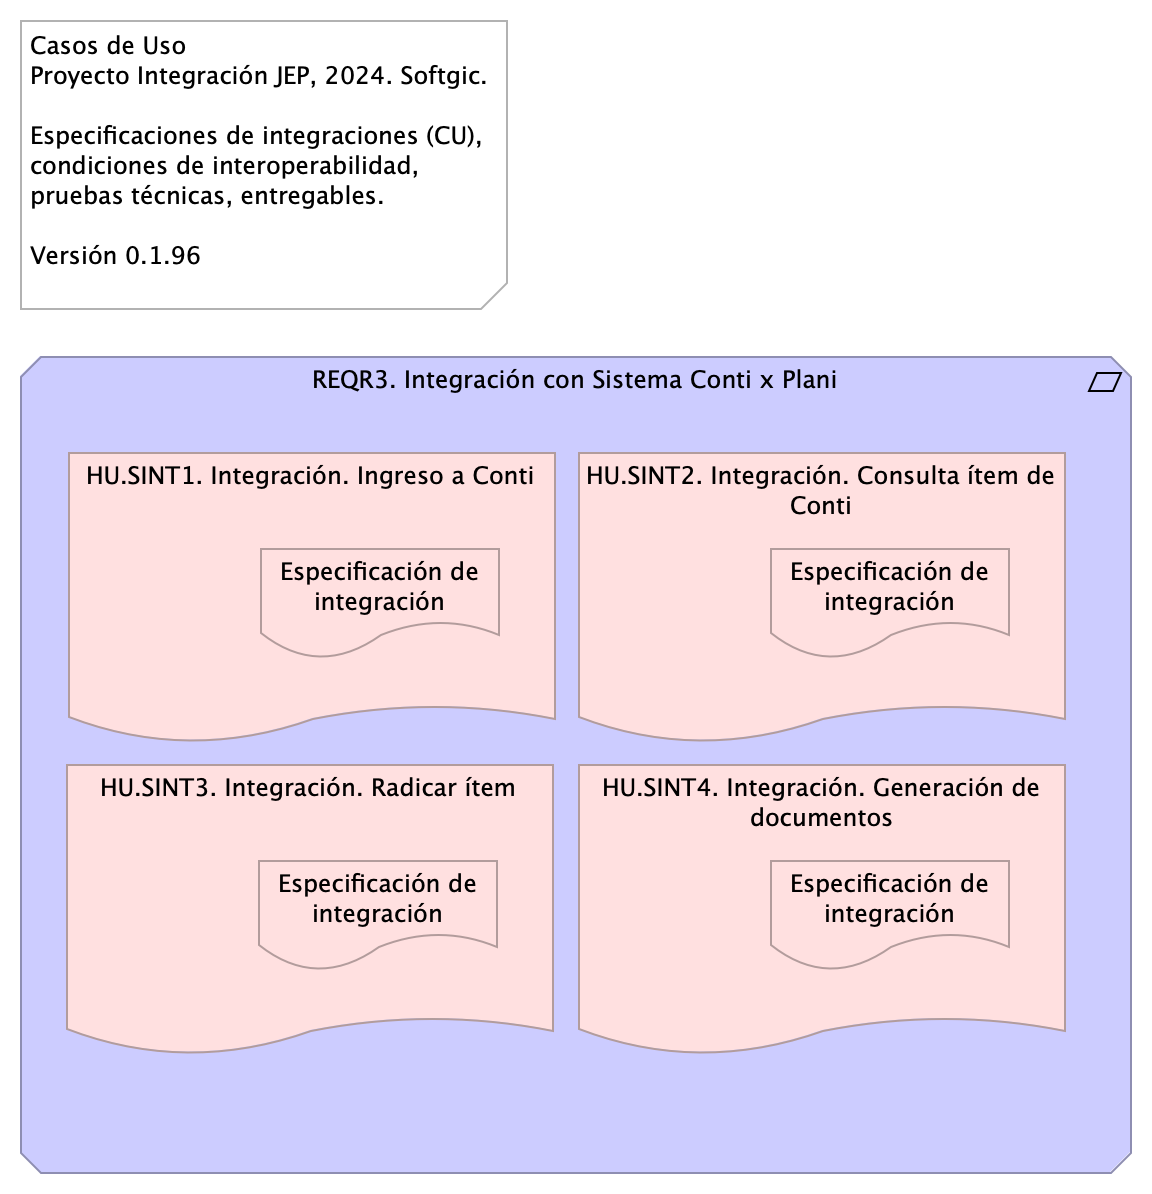
\includegraphics[width=\textwidth,height=5.20833in]{images/05.REQR.1n.4n.CasosdeUso.png}
\caption{05.REQR.1n.4n. Casos de Uso . \emph{Fuente: Repositorio
arquitectura Integración JEP
(2024)}}\label{fig:id-eb0cac3ffa954ca0aa6a48e757b4d309}
\end{figure}

\subsubsection{Catálogo de
Elementos}\label{sec:catuxe1logo-de-elementos}

\subsubsection{Especificación de
integración}\label{sec:especificaciuxf3n-de-integraciuxf3n}

Solicitar autenticación a la aplicación Conti y devolver resultado de la
solicitud de ingreso a la aplicación Plani.

\paragraph{Elementos}\label{sec:elementos}

Elegir y describir los elementos de la actual integración.

\begin{itemize}
\tightlist
\item[$\boxtimes$]
  App consumidora (A)
\item[$\boxtimes$]
  Mensaje
\item[$\square$]
  Canal
\item[$\square$]
  Ruteo
\item[$\square$]
  Traducción
\item[$\boxtimes$]
  App proveedora (B)
\item[$\square$]
  Monitoreo
\end{itemize}

Aplicación consumidora A: Plani. Aplicación proveedora B: Conti

Mensaje solicitud: (ver estándar de nombramiento) Ingreso a Conti

\begin{itemize}
\tightlist
\item
  Tipo: TXT \textbar{} SOAP \textbar{} XML \textbar{} JSN \textbar{} YML
  \textbar{} BASE64
\item
  Contenido: Usuario o identidad Conti
\end{itemize}

Mensaje respuesta: Rpta. Ingreso a Conti

\begin{itemize}
\tightlist
\item
  Tipo: TXT \textbar{} SOAP \textbar{} XML \textbar{} JSN \textbar{} YML
  \textbar{} BASE64
\item
  Contenido: Estado de solicitud de ingreso a Conti
\end{itemize}

Mensaje excepción: Rpta. Ingreso a Conti

\begin{itemize}
\tightlist
\item
  Tipo: TXT \textbar{} SOAP \textbar{} XML \textbar{} JSN \textbar{} YML
  \textbar{} BASE64
\item
  Contenido: Código de respuesta: HTTP 500 \textbar{} TXT \textbar{}
  Numeración (entero)
\end{itemize}

\paragraph{Diseño}\label{sec:diseuxf1o}

Message Construct \textbar{} Message Routing \textbar{} Message
Transformation \textbar{} Messaging Endpoints \textbar{} Messaging
Channels \textbar{} \ldots{}

La aplicación consumidora y proveedora compartirán capacidades mediante
un mensaje de autenticación (Message Construct).

\paragraph{Matriz de
interoperabilidad}\label{sec:matriz-de-interoperabilidad}

Detalle del intercambio entre sistemas de información o aplicaciones.

App Plani requiere compartir Información {[}I{]}, Funcionalidad {[}F{]},
Seguridad o Servicios {[}S{]} con la App Plani.

\begin{longtable}[]{@{}lllll@{}}
\caption{Matriz de interoperabilidad del CU Ingreso a
Conti.}\tabularnewline
\toprule\noalign{}
& Conti & Plani & Legali & Otros \\
\midrule\noalign{}
\endfirsthead
\toprule\noalign{}
& Conti & Plani & Legali & Otros \\
\midrule\noalign{}
\endhead
\bottomrule\noalign{}
\endlastfoot
Conti (B) & X & Seguridad & & \\
Plani (A) & & X & & \\
Legali & & & X & \\
Otros Sistemas & & & & X \\
\end{longtable}

\paragraph{Pruebas Realizables}\label{sec:pruebas-realizables}

Por cada caso de prueba de integración describir el resultado del
intercambio entre sistemas de información o aplicaciones según la Matriz
de interoperabilidad.

\begin{itemize}
\tightlist
\item
  PRUB1. Consumo: la aplicación consumidora Plani no recibe una
  respuesta a tiempo.
\item
  PRUB2. Ingreso: la aplicación proveedora Conti no provee un ingreso
  autorizado.
\end{itemize}

\subsubsection{Especificación de
integración}\label{sec:especificaciuxf3n-de-integraciuxf3n-1}

Solicitar consulta de ítem a la aplicación Plani y obtener resultado de
la consulta. La solicitud de consulta podrá realizarla con mínimo un
parámetro, o la combinación de todos. Los parámetros son los siguientes:

\begin{enumerate}
\def\labelenumi{\arabic{enumi}.}
\tightlist
\item
  Número de ítem
\item
  Fecha estimada de inicio de proceso de selección
\item
  Vigencia de ejecución
\item
  Fuente de los recursos
\item
  Modalidad de selección Interna (manual de contratación)
\end{enumerate}

Esta integración permitirá que el sistema Conti consulte al sistema
Plani la información de acuerdo con los campos solicitados. Cuando la
aplicación Plani ejecute la consulta enviará, esta integración enviarea
de regreso a Conti la lista de ítems relacionados que ya se encuentren
en estado aprobado y que correspondan a la dependencia del usuario
parametrizado en Conti.

\paragraph{Elementos}\label{sec:elementos-1}

Elegir y describir los elementos de la actual integración.

\begin{itemize}
\tightlist
\item[$\boxtimes$]
  App consumidora (A)
\item[$\boxtimes$]
  Mensaje
\item[$\boxtimes$]
  Canal
\item[$\square$]
  Ruteo
\item[$\boxtimes$]
  Traducción
\item[$\boxtimes$]
  App proveedora (B)
\item[$\square$]
  Monitoreo
\end{itemize}

Aplicación consumidora A: Conti. Aplicación proveedora B: Plani

Mensaje solicitud: (ver estándar de nombramiento) Consulta ítem

\begin{itemize}
\tightlist
\item
  Tipo: TXT \textbar{} SOAP \textbar{} XML \textbar{} JSN \textbar{} YML
  \textbar{} BASE64
\item
  Contenido: Estructura de datos consulta ítem
\end{itemize}

\begin{enumerate}
\def\labelenumi{\arabic{enumi}.}
\tightlist
\item
  Número de ítem
\item
  Fecha estimada de inicio de proceso de selección
\item
  Vigencia de ejecución
\item
  Fuente de los recursos
\item
  Modalidad de selección Interna (manual de contratación)
\end{enumerate}

Mensaje respuesta: Rpta. Ingreso a Conti

\begin{itemize}
\tightlist
\item
  Tipo: TXT \textbar{} SOAP \textbar{} XML \textbar{} JSN \textbar{} YML
  \textbar{} BASE64
\item
  Contenido: Estructura de datos ítem aprobado
\end{itemize}

\begin{enumerate}
\def\labelenumi{\arabic{enumi}.}
\tightlist
\item
  Vigencia de ejecución
\item
  ítem PAA
\item
  Fuente de los recursos
\item
  Valor Total Estimado del Contrato 5. Código UNSPSC
\item
  Objeto
\item
  Fecha estimada de inicio de proceso de selección(mes
\item
  Fecha estimada de presentación de ofertas (mes)
\item
  Duración estimada del contrato
\item
  Duración estimada del contrato (intervalo: días, meses, años)
\item
  Modalidad de selección Interna
\item
  Modalidad SECOPII
\item
  Departamento
\item
  Municipio
\item
  Dependencia
\item
  Responsable
\item
  Ordenador del gasto
\item
  Correo electrónico responsable
\end{enumerate}

Mensaje excepción: Rpta. Ingreso a Conti

\begin{itemize}
\tightlist
\item
  Tipo: TXT \textbar{} SOAP \textbar{} XML \textbar{} JSN \textbar{} YML
  \textbar{} BASE64
\item
  Contenido: Código de respuesta: ej. HTTP 500 \textbar{} TXT \textbar{}
  Numeración (entero)
\end{itemize}

\paragraph{Diseño}\label{sec:diseuxf1o-1}

Message Construct \textbar{} Message Routing \textbar{} Message
Transformation \textbar{} Messaging Endpoints \textbar{} Messaging
Channels \textbar{} \ldots{}

La aplicación consumidora y proveedora compartirán capacidades mediante
un canal centralizado, y mensajes de intercambio de información
transformada de extremo a extremo. (Message Construct, Message Routing,
Message Transformation, Messaging Endpoints).

\paragraph{Matriz de
interoperabilidad}\label{sec:matriz-de-interoperabilidad-1}

Detalle del intercambio entre sistemas de información o aplicaciones.

App Plani requiere compartir Información {[}I{]}, Funcionalidad {[}F{]},
Seguridad o Servicios {[}S{]} con la App Plani.

\begin{longtable}[]{@{}lllll@{}}
\caption{Matriz de interoperabilidad del CU Consulta
ítem.}\tabularnewline
\toprule\noalign{}
& Conti (A) & Plani (B) & Legali & Otros \\
\midrule\noalign{}
\endfirsthead
\toprule\noalign{}
& Conti (A) & Plani (B) & Legali & Otros \\
\midrule\noalign{}
\endhead
\bottomrule\noalign{}
\endlastfoot
Conti (A) & X & Información & & \\
Plani (B) & & X & & \\
Legali & & & X & \\
Otros Sistemas & & & & X \\
\end{longtable}

\paragraph{Pruebas Realizables}\label{sec:pruebas-realizables-1}

Por cada caso de prueba de integración describir el resultado del
intercambio entre sistemas de información o aplicaciones según la Matriz
de interoperabilidad.

\begin{itemize}
\tightlist
\item
  PRUB1.0 Consumo: la aplicación consumidora Conti no recibe la
  respuesta de la consulta a tiempo.
\item
  PRUB11. Consulta sin resultado: la aplicación proveedora Plani entrega
  una respuesta vacía.
\item
  PRUB12. Consulta incorrecta: la aplicación proveedora Plani no provee
  el formato de respuesta esperado.
\end{itemize}

\subsubsection{Especificación de
integración}\label{sec:especificaciuxf3n-de-integraciuxf3n-2}

Esta integracieon inicia en Conti el proceso de gestión dentro de la
ruta precontractual (Revisar documento ``1. Acta de requerimientos
Proceso Precontractual\_V2''), y pedirá un radicado asociado al ítem
seleccionado.

Una vez generado el número del radicado, Conti envía a Plani la llamada
posterior (callback) con esta información para que pueda ser almacenada
y relacionada al ítem en el sistema Plani. A su vez, Plani envía un
mensaje de confirmación a Conti.

\paragraph{Elementos}\label{sec:elementos-2}

Elegir y describir los elementos de la actual integración.

\begin{itemize}
\tightlist
\item[$\boxtimes$]
  App consumidora (A)
\item[$\boxtimes$]
  Mensaje
\item[$\boxtimes$]
  Canal
\item[$\boxtimes$]
  Ruteo
\item[$\boxtimes$]
  Traducción
\item[$\boxtimes$]
  App proveedora (B)
\item[$\square$]
  Monitoreo
\end{itemize}

Aplicación consumidora A: Conti. Aplicación proveedora B: Plani, C: Otro

Mensaje solicitud: (ver estándar de nombramiento) Consulta ítem

\begin{itemize}
\tightlist
\item
  Tipo: TXT \textbar{} SOAP \textbar{} XML \textbar{} JSN \textbar{} YML
  \textbar{} BASE64
\item
  Contenido: Estructura de datos consulta ítem
\end{itemize}

Mensaje respuesta: Rpta. Ingreso a Conti

\begin{itemize}
\tightlist
\item
  Tipo: TXT \textbar{} SOAP \textbar{} XML \textbar{} JSN \textbar{} YML
  \textbar{} BASE64
\item
  Contenido: Estructura de datos ítem aprobado
\end{itemize}

Mensaje excepción: Rpta. Ingreso a Conti

\begin{itemize}
\tightlist
\item
  Tipo: TXT \textbar{} SOAP \textbar{} XML \textbar{} JSN \textbar{} YML
  \textbar{} BASE64
\item
  Contenido: Código de respuesta: ej. HTTP 500 \textbar{} TXT \textbar{}
  Numeración (entero)
\end{itemize}

\paragraph{Diseño}\label{sec:diseuxf1o-2}

Message Construct \textbar{} Message Routing \textbar{} Message
Transformation \textbar{} Messaging Endpoints \textbar{} Messaging
Channels \textbar{} \ldots{}

La aplicación consumidora y proveedora compartirán capacidades mediante
un canal centralizado, y mensajes de intercambio de funcionalidad y
datos transformados de extremo a extremo. (Message Construct, Message
Routing, Message Transformation, Messaging Endpoints).

\paragraph{Matriz de
interoperabilidad}\label{sec:matriz-de-interoperabilidad-2}

Detalle del intercambio entre sistemas de información o aplicaciones.

App Plani requiere compartir Información {[}I{]}, Funcionalidad {[}F{]},
Seguridad o Servicios {[}S{]} con la App Plani.

\begin{longtable}[]{@{}lllll@{}}
\caption{Matriz de interoperabilidad del CU Radicar
ítem.}\tabularnewline
\toprule\noalign{}
& Conti (A) & Plani (B) & Legali & Otros (C) \\
\midrule\noalign{}
\endfirsthead
\toprule\noalign{}
& Conti (A) & Plani (B) & Legali & Otros (C) \\
\midrule\noalign{}
\endhead
\bottomrule\noalign{}
\endlastfoot
Conti (A) & X & Información & & Funcionalidad \\
Plani (B) & & X & & \\
Legali & & & X & \\
Otros Sistemas & & & & X \\
\end{longtable}

\paragraph{Pruebas Realizables}\label{sec:pruebas-realizables-2}

Por cada caso de prueba de integración describir el resultado del
intercambio entre sistemas de información o aplicaciones según la Matriz
de interoperabilidad.

\begin{itemize}
\tightlist
\item
  PRUB20 Consumo: la aplicación consumidora Conti no recibe la respuesta
  del radicado a tiempo.
\item
  PRUB21. Radicado: la aplicación proveedora del radicado falla en
  proveer el radicado
\item
  PRUB22. Consulta incorrecta: la aplicación proveedora Plani no provee
  el formato de respuesta esperado.
\end{itemize}

\subsubsection{Especificación de
integración}\label{sec:especificaciuxf3n-de-integraciuxf3n-3}

Una vez se tenga seleccionado el ítem a gestionar el usuario debe
identificar el tipo de documento que esté relacionado al mismo, sea
documento justificativo, Reglas de invitación y/o anexos.

Esta integración debe enviar el documento a\ldots{}

\paragraph{Elementos}\label{sec:elementos-3}

Elegir y describir los elementos de la actual integración.

\begin{itemize}
\tightlist
\item[$\square$]
  App consumidora (A)
\item[$\square$]
  Mensaje
\item[$\square$]
  Canal
\item[$\square$]
  Ruteo
\item[$\square$]
  Traducción
\item[$\square$]
  App proveedora (B)
\item[$\square$]
  Monitoreo
\end{itemize}

Aplicación consumidora A: Conti. Aplicación proveedora B:

Mensaje: Ingreso a Conti * Tipo: TXT \textbar{} SOAP \textbar{} XML
\textbar{} JSN \textbar{} YML \textbar{} BASE64 * Contenido:

\paragraph{Diseño}\label{sec:diseuxf1o-3}

Message Construct \textbar{} Message Routing \textbar{} Message
Transformation \textbar{} Messaging Endpoints \textbar{} Messaging
Channels \textbar{} \ldots{}

\paragraph{Matriz de
interoperabilidad}\label{sec:matriz-de-interoperabilidad-3}

Detalle del intercambio entre sistemas de información o aplicaciones.

App Plani requiere compartir Información {[}I{]}, Funcionalidad {[}F{]},
Seguridad o Servicios {[}S{]} con la App Plani.

\begin{longtable}[]{@{}lllll@{}}
\caption{Matriz de interoperabilidad del CU Generación de
documentos}\tabularnewline
\toprule\noalign{}
& Conti & Plani & Legali & Otros \\
\midrule\noalign{}
\endfirsthead
\toprule\noalign{}
& Conti & Plani & Legali & Otros \\
\midrule\noalign{}
\endhead
\bottomrule\noalign{}
\endlastfoot
Conti (B) & X & Información & & \\
Plani (A) & & X & & \\
Legali & & & X & \\
Otros Sistemas & & & & X \\
\end{longtable}

\paragraph{Pruebas Realizables}\label{sec:pruebas-realizables-3}

Por cada caso de prueba de integración describir el resultado del
intercambio entre sistemas de información o aplicaciones según la Matriz
de interoperabilidad.

\begin{itemize}
\tightlist
\item
  PRUB1.
\item
  PRUB2.
\end{itemize}

\subsubsection{HU.SINT1. Integración. Ingreso a
Conti}\label{sec:hu.sint1.-integraciuxf3n.-ingreso-a-conti}

\subsubsection{HU.SINT2. Integración. Consulta ítem de
Conti}\label{sec:hu.sint2.-integraciuxf3n.-consulta-uxedtem-de-conti}

\subsubsection{HU.SINT3. Integración. Radicar
ítem}\label{sec:hu.sint3.-integraciuxf3n.-radicar-uxedtem}

\subsubsection{HU.SINT4. Integración. Generación de
documentos}\label{sec:hu.sint4.-integraciuxf3n.-generaciuxf3n-de-documentos}

\subsubsection{REQR3. Integración con Sistema Conti x
Plani}\label{sec:reqr3.-integraciuxf3n-con-sistema-conti-x-plani}

Atendiendo la necesidad de la Subdirección de Contratación de
implementar el flujo de gestión precontractual en el sistema de Gestión
Documental - Conti se requiere contar con la información de los ítems
del Plan Anual de Adquisiciones -- PAA para iniciar el proceso, la cual
se encuentra gestionada en el Sistema de Gestión y Planeación
Institucional PLANi.

\subsubsection{Índice de la documentación (casos de
uso)}\label{sec:uxedndice-de-la-documentaciuxf3n-casos-de-uso}

\begin{enumerate}
\def\labelenumi{\arabic{enumi}.}
\tightlist
\item
  Integración. Ingreso a Conti
\item
  Integración. Consulta ítem de Conti
\item
  Integración. Radicar ítem 1.Integración. Generación de documentos
\end{enumerate}

\newpage

\section{Anexos}\label{sec:anexos}

\subsection{Plantilla de Casos de Uso del Proyecto
JEP}\label{sec:plantilla-de-casos-de-uso-del-proyecto-jep}

\begin{figure}
\centering
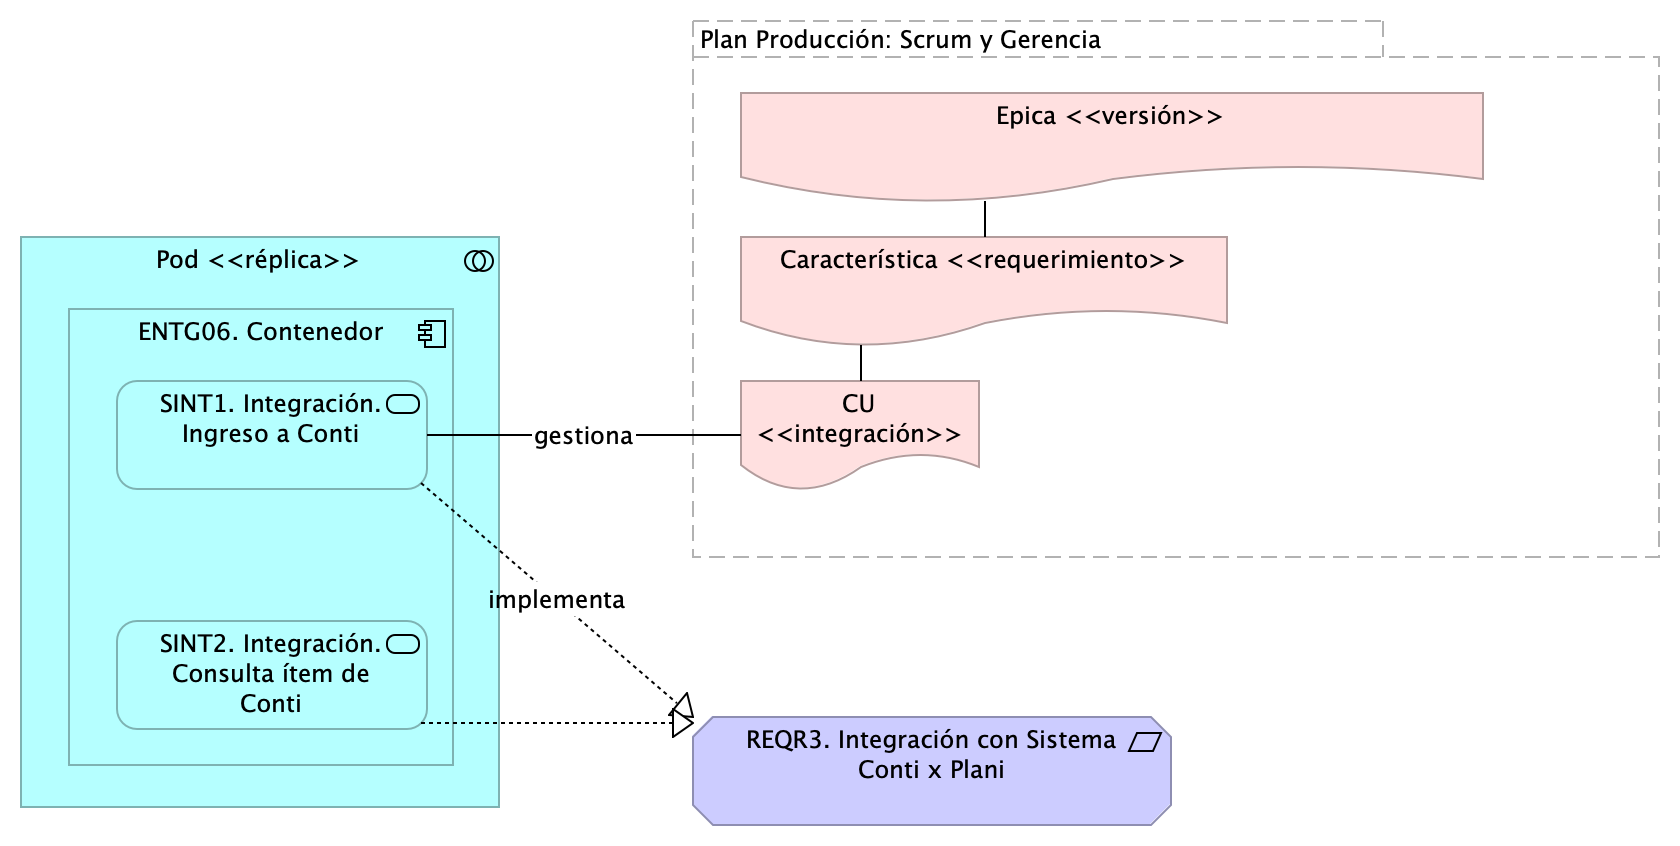
\includegraphics[width=\textwidth,height=5.20833in]{images/05.REQR.1n.3n.PlantillaCasodeUso.png}
\caption{05.REQR.1n.3n. Plantilla Caso de Uso. \emph{Fuente: Repositorio
arquitectura Integración JEP
(2024)}}\label{fig:id-8115cb4314954a7cb873b534038c22aa}
\end{figure}

Documentación de los casos de uso de integración (CU en el diagrama) del
proyecto JEP relacionados con las integraciones y requerimientos.

Fuente: Justificativo de la Contratación Invitación Pública.

\subsection{Casos de Uso del Proyecto
(integración)}\label{sec:casos-de-uso-del-proyecto-integraciuxf3n}

App A requiere integrar Información {[}I{]} \textbar{} Funcionalidad
{[}F{]} \textbar{} Servicios {[}S{]} con la App B, C, D\ldots{}

\subsubsection{Elementos}\label{sec:elementos-4}

Elegir y describir los elementos de la actual integración.

\begin{itemize}
\tightlist
\item[$\square$]
  App consumidora (A)
\item[$\square$]
  Mensaje
\item[$\square$]
  Canal
\item[$\square$]
  Ruteo
\item[$\square$]
  Traducción
\item[$\square$]
  App proveedora (B)
\item[$\square$]
  Monitoreo
\end{itemize}

\subsubsection{Diseño}\label{sec:diseuxf1o-4}

Message Construct \textbar{} Message Routing \textbar{} Message
Transformation \textbar{} Messaging Endpoints \textbar{} Messaging
Channels \textbar{} \ldots{}

\subsubsection{Matriz de
interoperabilidad}\label{sec:matriz-de-interoperabilidad-4}

Detalle del intercambio entre sistemas de información o aplicaciones.

Sistema A comparte información, funcionalidad o servicios con Sistema B.

\begin{longtable}[]{@{}lllll@{}}
\toprule\noalign{}
& Conti & Plani & Legali & Otros \\
\midrule\noalign{}
\endhead
\bottomrule\noalign{}
\endlastfoot
Conti & X & Inf, Seguridad & & \\
Plani & & X & & \\
Legali & & & X & \\
Otros Sistemas & & & & X \\
\end{longtable}

\subsubsection{Pruebas Realizables}\label{sec:pruebas-realizables-4}

Describir por cada caso de prueba de integración el resultado del
intercambio entre sistemas de información o aplicaciones según la Matriz
de interoperabilidad.

\end{document}
